\documentclass[12pt,a4paper]{article}
\usepackage[margin=25mm]{geometry}
\usepackage{amsmath,amssymb}
\usepackage{booktabs}
\usepackage{graphicx}
\usepackage{hyperref}
\usepackage{xcolor}
\usepackage{enumitem}
\usepackage{microtype}
\usepackage{caption}
\usepackage{array}
\usepackage{longtable}
\usepackage{lineno}

\hypersetup{colorlinks=true,linkcolor=blue!45!black,citecolor=blue!45!black,urlcolor=blue!55!black}
\setlist{nosep}
\emergencystretch=2em
\linenumbers

\newcommand{\workingnote}{%
  \begin{center}
  \fcolorbox{red!55!black}{red!4}{\parbox{0.92\linewidth}{\textbf{Working manuscript.}
  The external expert review of SAGA decision support has not been completed.
  The manuscript is therefore not ready for journal submission, and no placeholder
  effectiveness result may be interpreted as evidence.}}
  \end{center}}

\title{External validation and evidence-gated decision support for a virtual
hydrogen refuelling station digital twin}
\author{Author names withheld in working draft\\
\small Affiliation and corresponding-author details to be confirmed}
\date{Working draft: 3 October 2026}

\begin{document}
\maketitle
\workingnote

\begin{abstract}
This study separates evidence for process physics, consequence software and
language-model decision support in a virtual hydrogen station. A measured-boundary
Type-IV model was calibrated on 23 fills and evaluated on 12 frozen fills,
yielding pressure, temperature and state-of-charge root-mean-square errors of
3.841 MPa, 4.833 $^{\circ}$C and 3.850 percentage points; results did not transfer
to the full controller. A frozen 22-case PRESLHY blowdown evaluation failed:
50.0\% passed both screens versus 70\%, with six domain failures. A non-adiabatic
revision passed 20/22 consumed cases, but its E5.1 holdout was ineligible and
negative (2/3 primary passes). An independent 90 MPa campaign passed 0/3
mass-flow series. Two separately frozen Sandia/SRI transients failed their joint
mass-flow and pressure-decay screens; a third scaled-release trace passed all
screens. The consequence adapter matched HyRAM+ 6.1; identical source
passed 47 tests and 803 subtests. A blinded HIAD protocol is specified, but expert
ratings are pending. Evidence supports a claim-bounded prototype, not a
field-qualified controller or autonomous emergency system.
\end{abstract}

\noindent\textbf{Keywords:} hydrogen refueling station; digital twin; external
validation; HyRAM; process safety; decision support

\section{Introduction}
Hydrogen refuelling couples high-pressure storage, compression, cascade dispatch,
pre-cooling, flow control and vehicle-tank heat transfer. A useful digital twin
must conserve mass and energy, reproduce the fast-fill transient, expose safety
states and distinguish measured or simulated evidence from assumed inputs.
The physical decomposition follows the principal station elements in ISO
19880-1, while a conforming light-duty fuelling controller would additionally
require an authorized SAE J2601 implementation \cite{iso19880,saej2601}.
Published models have addressed vehicle filling and partial or whole-station
dynamics, including the H2FillS formulation \cite{kuroki2021}, optimization of
cascade refuelling \cite{rothuizen2013}, vehicle-side pressure loss
\cite{rothuizen2020}, and multi-zone tank heat transfer \cite{xiao2024}. These
works also show why agreement at one component boundary cannot establish the
accuracy of an entire station controller.
Independent field evidence is available at a coarser resolution. An NRC Canada
analysis of approximately 22,593 H70T40 dispensing events at four British
Columbia stations reports protocol context, normal/incomplete/fault-fill
categories and plotted pressure, temperature and flow patterns
\cite{nrc2024}. The report does not release synchronized machine-readable logs,
so we use it for operating-range and fault-taxonomy context rather than as a
numerical full-loop holdout.

The public PRHYDE deliverable provides a broader protocol and experiment
context: four instrumented tanks (240 L H70, 350 L H50, 322 L H35 and 165 L
H70) were tested at ZBT and Nikola across pressure-ramp and delivery-
temperature conditions \\cite{prhyde2023}. Its public artifact contains test
matrices, plots and aggregate model errors, but not the synchronized logger
arrays needed for an untouched numerical holdout. An earlier JHFC/NEDO study
likewise reports six practical 35/70 MPa filling conditions and station-supplied
pressure/temperature measurements \\cite{monde2012}; the current public article
and project archive do not expose the underlying machine-readable runs. These
sources therefore support operating-range context and data-request targeting,
not a new external pass claim.

Safety-oriented twins add a second model family. Release, dispersion, jet-fire,
overpressure and quantitative-risk calculations are commonly delegated to a
consequence package such as HyRAM+ \cite{hyram2024,hyram2025}. A third layer now
uses large language models (LLMs) to turn process and consequence results into
operator-facing explanations. The layers have different evidence requirements.
Passing unit tests cannot validate thermodynamics; matching a public consequence
API cannot validate site geometry; and fluent text cannot demonstrate safe or
useful advice.

This work asks five separate questions:
\begin{enumerate}
  \item How accurately does the vehicle-tank submodel reproduce public fast-fill
  experiments when measured boundary conditions are imposed?
  \item Does the complete controller--cascade--precooler--vehicle loop meet
  predeclared engineering error screens?
  \item Does the source-depletion and direct-aperture model meet prospectively
  specified screens on independent ambient hydrogen blowdown experiments?
  \item Does the production adapter preserve the inputs and outputs of the exact
  installed HyRAM+ package?
  \item Can process- and evidence-linked SAGA responses improve incident decision
  support relative to deterministic alarms without increasing unsafe advice?
\end{enumerate}
The first four questions have reproducible results. The fifth has a frozen
protocol but no external expert result at the time of this draft.

\section{Materials and methods}
\subsection{Digital-twin boundary}
The virtual station represents tube-trailer supply, a three-stage compressor,
low-, medium- and high-pressure storage banks, two independently dispatched
dispenser circuits, pre-cooling, hose line-pack and Type-IV vehicle vessels.
Sampled supervisory and safety logic is coupled to continuous mass and energy
balances. Process operations remain event-driven: the state is held when no
transfer, compression, venting or incident request is active. The visual scene,
simulated sensors and emergency-action interface are research and training
components; they are not an as-built survey or a certified safety instrumented
system.

The process model owns pressure, temperature, inventory and mass flow. A release
snapshot, including source state and explicitly selected aperture, is passed to
the consequence layer. The LLM is called only after deterministic process,
alarm and available consequence fields have been assembled. Sensor analysis,
the main conversational interface and the separate SAGA retrieval service have
isolated API contracts so that a command request is not silently replaced by a
periodic status report.

\subsection{Vehicle-tank model}
The Type-IV surrogate uses gas, liner and composite-shell energy states. For gas
mass $m_g$, gas internal energy $U_g$ and effective volume $V_{\mathrm{eff}}$,
real-gas properties close the state through density and specific internal energy:
\begin{align}
 \rho_g &= m_g/V_{\mathrm{eff}}, & u_g &= U_g/m_g,\\
 (p_g,T_g,h_g) &= \mathcal{P}_{\mathrm{H_2}}(\rho_g,u_g).
\end{align}
The property operator $\mathcal{P}_{\mathrm{H_2}}$ is implemented with CoolProp;
no ideal-gas density substitution is used. The balances are
\begin{align}
 \frac{dm_g}{dt} &= \dot m_{\mathrm{in}}-\dot m_{\mathrm{out}},\\
 \frac{dU_g}{dt} &= \dot m_{\mathrm{in}}h_{\mathrm{in}}
 -\dot m_{\mathrm{out}}h_g-UA_{gl}(T_g-T_l),\\
 C_l\frac{dT_l}{dt} &= UA_{gl}(T_g-T_l)-UA_{ls}(T_l-T_s),\\
 C_s\frac{dT_s}{dt} &= UA_{ls}(T_l-T_s)-UA_{sa}(T_s-T_{\mathrm{amb}}).
\end{align}
The fixed volume is scaled from 0.122 m$^3$ per 4.7 kg nominal capacity because
machine-readable vessel geometry was not present in the public overview. This is
an explicit source of structural uncertainty.

\subsection{Public fast-fill data and frozen split}
Five checksum-verified archives from H2Protocol/Powertech Labs were normalized
into 36 SAE J2601 Tables Method fills \cite{schneider2014}. The model uses the
experimental clock and is interpolated to measured timestamps without dynamic
time warping. An experiment-only mass-closure screen compares integrated measured
flow with the nominal inventory change inferred from reported state of charge
(SOC). The admissible ratio was fixed at 0.8--1.2; one repeat-fill case was
excluded because its ratio was 1.428. This screen contains no model prediction.

Closed-loop mass-flow timing diagnostics subsequently exposed a normalization
error in development case H2P-L29. An isolated 1.526 g s$^{-1}$ pulse at workbook
time zero caused the former first/last-threshold rule to prepend 369.5 s of idle
data to the sustained fill. A disclosed amendment clusters above-threshold samples
using a 15 s maximum gap, discards terminal clusters below the larger of 0.005 kg
or 0.2\% of clustered mass, and preserves meaningful multi-segment fills and their
internal gaps. The corrected H2P-L29 trace contains 399 samples over 199 s instead
of 1,143 samples over 571 s. All tank results below were regenerated after this
correction; the earlier normalization is superseded.

Every third laboratory test (3, 6, \ldots, 36) forms a frozen 12-fill validation
set. The remaining 23 admissible fills estimate two global parameters: effective
volume multiplier and gas-to-liner heat-transfer multiplier. The fitted values
were 1.05273 and 31.46066, respectively. Optimization used bounded nonlinear
least squares in log-parameter space. No case-specific parameter was fitted.
Case-level uncertainty was estimated with 10,000 nonparametric bootstrap
resamples using seed 2601.

As an independent operating-range reference, the 3Emotion programme reports
multi-year operator logs from five 350-bar bus refuelling stations and 34 buses,
including aggregate fill mass, duration, average flow, availability and
utilisation indicators \cite{caponi2022}. The reported overall means (14.62 kg
per fill and 10.28 min) are retained in the repository's public-data inventory
as an aggregate benchmark. They are not used as a synchronized time-series
holdout: the public record does not release common-time-base pressure,
temperature, mass-flow and valve-state rows. This distinction prevents an
operating-range comparison from being presented as full-loop physics
validation.

For a variable $y$ with $n$ aligned samples, the principal metric is
\begin{equation}
 \mathrm{RMSE}(y)=\sqrt{\frac{1}{n}\sum_{i=1}^{n}
  (y_i^{\mathrm{model}}-y_i^{\mathrm{measured}})^2}.
\end{equation}
Pressure, gas temperature and density-based SOC were evaluated separately.

\subsection{Complete closed-loop evaluation}
The full loop adds a sampled pressure-ramp controller, PI flow command, cascade
selection, finite valve motion, line-pack, precooling and station-to-vehicle
hydraulics. The global tank parameters were frozen before this evaluation. A
development-only adaptive search selected one dispenser flow-area multiplier of
2.0 on eight declared development fills; the initial grid was extended only after
its optimum fell at the upper bound. Density-based SOC used each experiment's
nominal 35 or 70 MPa working pressure.

Initial comparison exposed three structural errors: flow-limited anti-windup
could reverse the integral while pressure error remained positive; a fixed
$-20\,^{\circ}$C precooler trip stopped warmer delivery classes; and cascade
selection could regress to a lower bank. The corrected implementation uses
conditional-integration anti-windup, a delivery-class-dependent trip while
preserving the default T40 limit, monotonic low-to-medium-to-high dispatch, and
independent dispatch state for the two dispenser circuits. No fitted parameter
was changed after these corrections.

Engineering screens were fixed at pressure RMSE $\leq5$ MPa, temperature RMSE
$\leq10\,^{\circ}$C and absolute final SOC error $\leq5$ percentage points. These
are project screens, not SAE conformance limits. Eleven comparison fills had
already been inspected before the structural repair; their later results are
therefore internal confirmation rather than an untouched holdout.

An additional Powertech Labs MC Default bench-test archive was then used as a
prospective external holdout. Before any selected workbook outcome was opened,
the archive SHA-256, eight eligible workbook paths, model commit, fitted tank
parameters, dispenser multiplier, exclusion rules and the three engineering
screens were committed. The frozen controller accepts one constant APRR, whereas
the publisher supplies a pressure--time schedule. We therefore mapped each
schedule to its endpoint-equivalent average pressure ramp. This disclosed
approximation tests transportability of the frozen implementation; it is not an
implementation or certification of the proprietary MC Formula. No case-specific
fit, post-freeze tuning, dynamic time warping or failed-case exclusion was
permitted.

\subsection{Prospective ambient blowdown validation}
The source-depletion and direct-aperture release model was independently evaluated
with the PRESLHY E3.1 DisCha dataset \cite{preslhy2023}. Before any numerical Excel
outcome was opened, the protocol and implementation hashes, inclusion rules,
pressure interpretation, time alignment, endpoints, thresholds, bootstrap seed
and negative-result policy were committed. The evaluation included all eligible
300 K workbooks from the 0.5, 1, 2 and 4 mm packages. The facility has a 2.815 L
stainless-steel vessel; initial absolute pressure and internal gas temperature
were taken from measured channels. Because the selected workbooks contain no
ambient-pressure channel, 101.325 kPa was substituted and flagged. A terminal
near-zero vessel-pressure signal was interpreted as gauge pressure. Published
synchronized time, whose zero is the first significant nozzle-line pressure rise,
was retained without fitted shift or time warping.

The frozen model used a rigid adiabatic 2.815 L control volume, instantaneous full
opening, nominal circular aperture and pre-existing discharge coefficient 0.8.
It did not model vessel-wall heat transfer, valve travel, release-line inventory,
pipe backpressure or two-phase flow. Evaluation began at 0.1 s and ended at the
first measured pressure at or below 1.05 times ambient or the record end. The two
case screens were pressure NRMSE no greater than 10\% of initial absolute pressure
and time-to-50\%-initial-gauge-pressure relative error no greater than 20\%.
At least 12 cases spanning three nozzle and three pressure groups were required;
the aggregate claim required at least 70\% to pass both screens. The case was the
unit for 10,000 bootstrap resamples with seed 20261003. Eligible integration or
property-domain failures were retained as failed cases.

The negative E3.1 result was followed by a development-only revision. It used a
real-gas equation of state, maximum isentropic mass flux, the published 28 kg
stainless-steel wall, a lumped wall energy balance, Churchill--Chu internal
natural convection and a 6 W m$^{-2}$ K$^{-1}$ external coefficient. The global
discharge coefficient remained 0.8 and no case-specific fitting was allowed.
Because the same 22 records informed this revision, its performance is diagnostic
rather than confirmatory. The model and evaluator were then hash-locked before
numerical access to the separate PRESLHY E5.1 ignited-discharge campaign
\cite{preslhye5}. The primary window required measured initial gas temperature
280--330 K, initial pressure 0.5--21 MPa, at least four experiments, two nozzle
groups and two pressure groups. The original two case screens and 70\% aggregate
rule were retained. Complete source-pressure traces, including post-ignition
samples, were evaluated; failed integrity or model evaluations were retained.

A second transfer test used the independent INERIS/CEA 25 L Type-IV campaign
near 90 MPa \cite{proust2011}. Before numerical figure values were read, the
model, evaluator, three-series minimum and endpoints were hash-locked. Figure 5
mass-flow curves were digitized independently from PDF vector paths and a 4x
raster render; their mean was retained and half their difference plus half-pixel
resolution defined digitization uncertainty. Table 1 supplied measured source
temperature at the same pressure states. The primary window was 2--95 MPa,
220--330 K and at least eight states in each of the 1, 2 and 3 mm series. Series
screens were mass-flow NRMSE no greater than 15\% of measured peak and median
absolute percentage error no greater than 20\%; at least two of all three
eligible diameter series had to pass. The pressure axis was treated as absolute;
adding 101.325 kPa was predeclared as a non-controlling basis sensitivity.

A third transfer test used the independent Sandia/SRI blowdown reported by
Schefer et al. \cite{schefer2006} and the experimental Figure 3b coordinates
distributed with HyRAM+ 6.1. The evaluator and endpoints were committed before
any numerical coordinate was opened, although an approximate 100 s total
duration was already visible in secondary descriptions and was disclosed. The
locked model was a well-mixed adiabatic 0.098 m$^3$ vessel, initially at
15.513 MPa and 315.15 K, discharging through the published 3.175 mm controlling
manifold restriction with the public HyRAM+ benchmark value $C_d=1.0$. At least
15 points were required. All three screens had to pass: peak-normalized mass-flow
NRMSE $\leq15\%$, median absolute percentage error $\leq20\%$ above 10\% of
measured peak, and half-peak-time error $\leq20\%$.

A fourth transfer test used the different 2007 Sandia/SRI pressure-decay
experiment \cite{schefer2007}. Its evaluator, code and data hash were committed
before any numerical Figure 4 coordinate was opened. The locked model was a
well-mixed adiabatic 1.234 m$^3$ vessel initially at 43.1 MPa and 290 K,
discharging through the published 5.08 mm restriction with $C_d=1.0$. At least
15 points were required. All three screens had to pass: initial-pressure-
normalized RMSE $\leq10\%$, median absolute percentage error $\leq15\%$ above
10\% of initial pressure, and half-pressure-time error $\leq20\%$.

A fifth transfer test used the scaled hydrogen release from Ekoto et al.
\cite{ekoto2012}. Its evaluator, code and data hash were likewise committed
before numerical Figure 3 coordinates were opened. Public apparatus inputs were
13.45 MPa, 297 K, 3.63 L, a 3.56 mm restriction and $C_d=0.75$. The mass-flow
NRMSE, median error and half-peak-time limits were the same 15\%, 20\% and 20\%
screens used for the 2006 transient, and all three were required.

\subsection{Consequence-model verification}
HyRAM+ receives immutable release state and geometry from the twin. The
production adapter reports (i) the directional centreline distance to 4 vol\%
hydrogen for an unignited jet, (ii) sampled 5 kW m$^{-2}$ jet-fire heat flux and
(iii) sampled 5 kPa unconfined overpressure. The latter two distances are bounded
by the configured observation coordinates and are not regulatory setbacks.

Verification used the exact public HyRAM+ v6.1 tag and commit
\texttt{b45abf9a6d99\allowbreak 5951311be6aa\allowbreak d836f1874e4d\allowbreak 420b}.
Installed Python-source hashes
were compared with the clone. Sandia's upstream plume, heat-flux and unconfined
overpressure validation tests were executed unchanged. Three station-scale parity
cases then called both the production adapter and the public HyRAM API and compared
every translated field with relative tolerance $10^{-12}$ and absolute tolerance
$10^{-9}$. A separate display contract preserves the sampled thermal/blast radius,
the directional 4 vol\% plume length and width, and the release angle without unit
conversion. Browser regression tests prevent these physically different quantities
from being collapsed into one spherical extent.

\subsection{Incident decision-support evaluation}
The incident study population is the hydrogen-refuelling-station subset of the
European Commission JRC HIAD 2.2 database \cite{hiad2026}. Of 34 identified HRS events, 33 contain
at least one emergency action, lesson or corrective field. Only a coordinator-
approved historical observation is supplied to the system; recorded response and
lesson fields are withheld as reviewer reference material. A deterministic
pre-screen highlights exact phrase overlap and possible completed-response
sentences but cannot approve a case. A non-rating coordinator must inspect all
holdout vignettes; the approved input is then checked against the original case
set and SHA-256 locked before response collection.
For broader actual-accident provenance, the response catalog also links 23 public
KHK hydrogen accident reports covering 26 incident codes and eight precaution
reports \cite{khk2026}. URL-level checks confirmed PDF availability and recorded
hashes and page counts without mirroring report files or text; these records are
used for qualitative scenario grounding only and are excluded from numerical
physics or frequency claims.

The frozen protocol compares a deterministic alarm, three direct one-pass SAGA
responses and three SAGA responses with standards-document retrieval. Output is
masked and randomized. Three independent reviewers with documented
hydrogen/process-safety experience score situation accuracy, immediate-action
correctness, priority, stabilization/restart, prevention, evidence grounding and
operator usability from 1 to 5. Critical omission and unsafe advice are separate
binary endpoints. The event is the unit of inference. Repeats and reviewers are
averaged within event before paired bootstrap confidence intervals and Wilcoxon
signed-rank comparisons are calculated. Failed provider calls remain as masked
failure responses for scoring rather than being removed or silently retried.
Because the 24-event holdout is fixed by the eligible public-incident population,
a seeded pre-outcome sensitivity simulation reports Wilcoxon power over standardized
paired effects. Repeats do not increase the inferential event count, and a zero-event
exact upper confidence bound is retained for unsafe-advice outcomes.
No LLM-as-judge score is accepted as the
primary endpoint. Holdout responses and ratings have not yet been collected.
The applicable institutional ethics determination for expert-participant research
must be recorded before reviewer recruitment or rating collection.

\section{Results}
\subsection{Measured-boundary tank validation}
Table~\ref{tab:tank} reports the frozen split. Validation errors were lower than
calibration means for all three primary quantities, although uncertainty remains
wide across heterogeneous fill conditions. Figure~\ref{fig:parity} shows aligned
pressure and temperature predictions; Figure~\ref{fig:cases} exposes the
case-to-case error distribution rather than only an aggregate value.

\begin{table}[htbp]
\centering
\caption{Type-IV tank-model results. Parentheses are case-bootstrap 95\% confidence intervals for the mean.}
\label{tab:tank}
\small
\resizebox{\textwidth}{!}{%
\begin{tabular}{lrrrr}
\toprule
Split & Cases & Pressure RMSE & Temperature RMSE & SOC RMSE \\
 & & (MPa) & ($^{\circ}$C) & (percentage points) \\
\midrule
Calibration & 23 & 4.529 (3.237--6.126) & 7.889 (6.072--9.870) & 4.455 (3.517--5.455) \\
Validation & 12 & 3.841 (2.507--5.835) & 4.833 (3.707--6.113) & 3.850 (2.921--4.909) \\
\bottomrule
\end{tabular}
}
\end{table}

\begin{figure}[htbp]
\centering
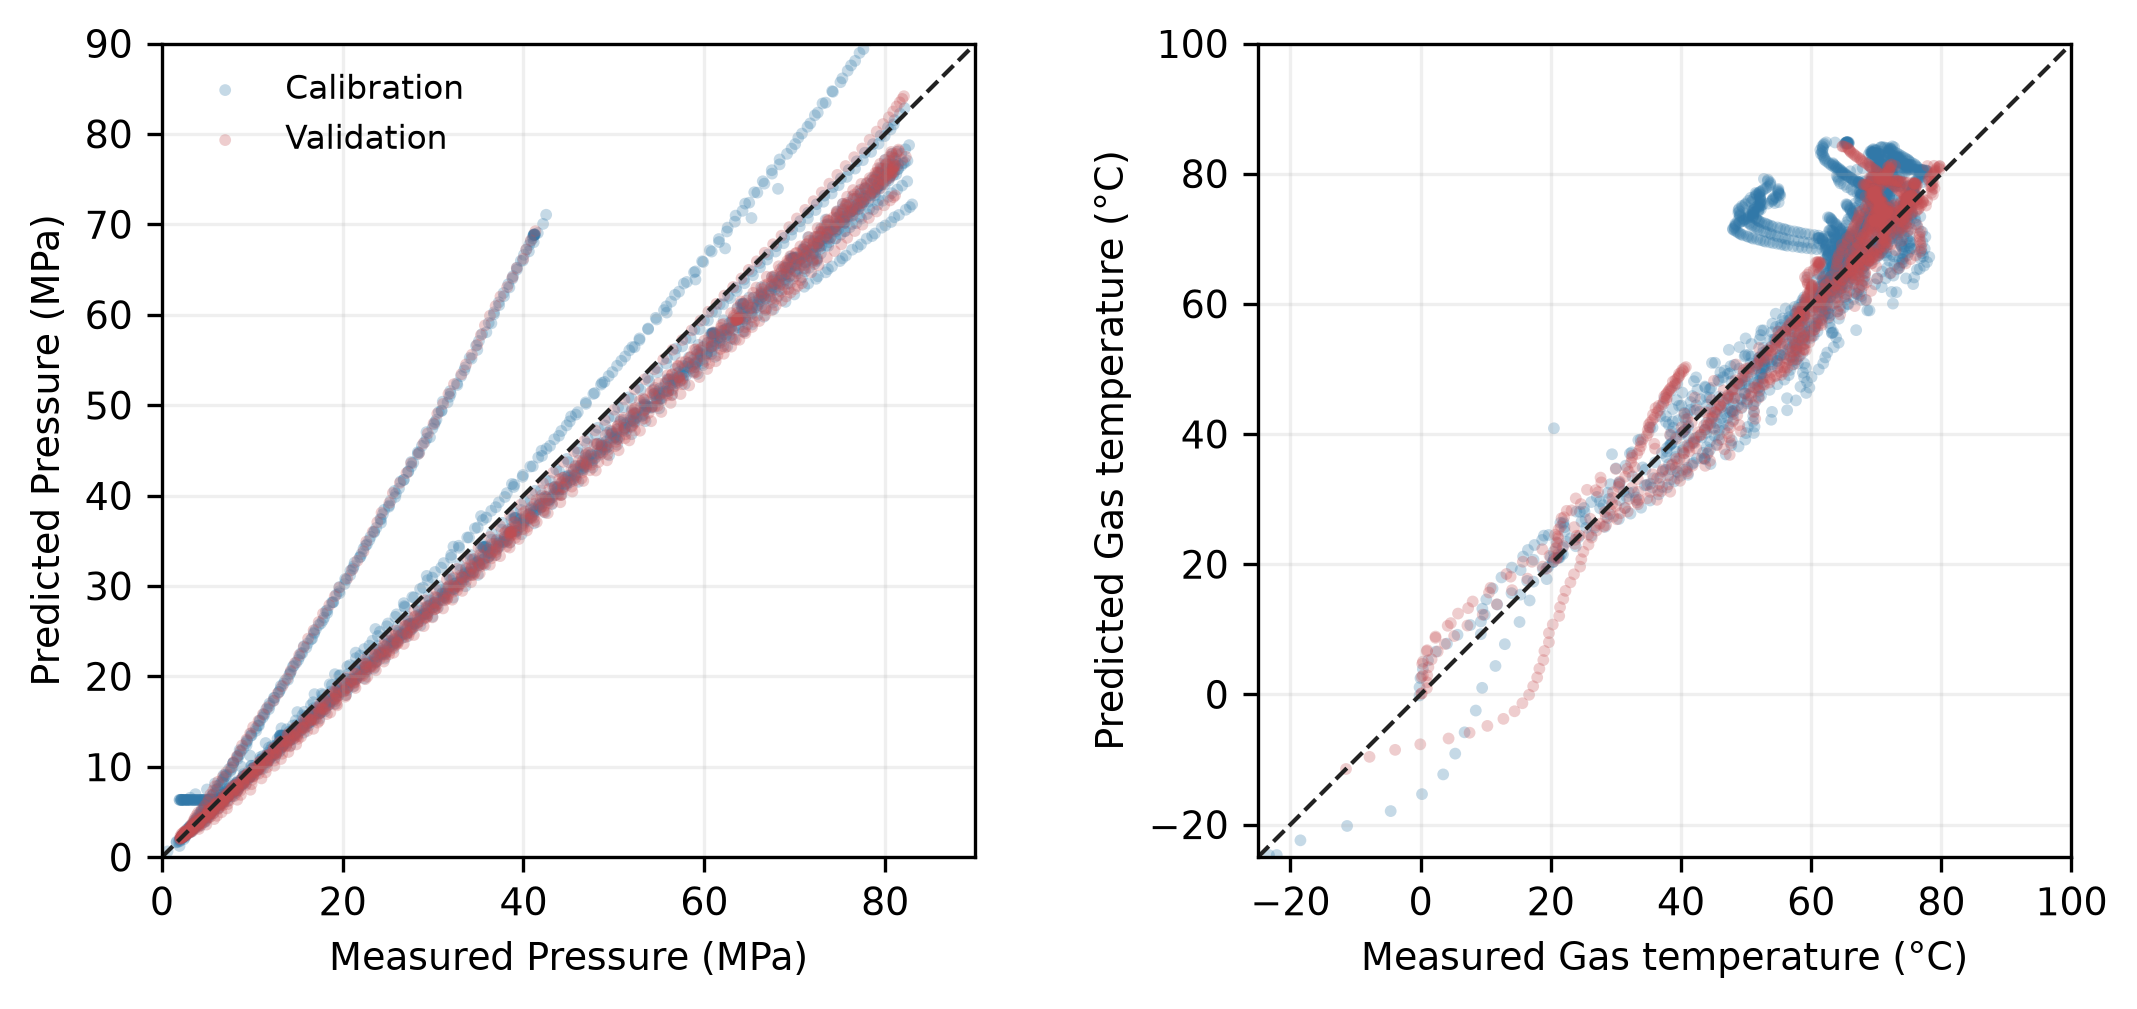
\includegraphics[width=\linewidth]{figures/tank_parity.png}
\caption{Measured and predicted tank pressure and gas temperature on the
experimental time bases. Points are semi-transparent so repeated trajectories
remain visible. The dashed line denotes equality.}
\label{fig:parity}
\end{figure}

\begin{figure}[htbp]
\centering
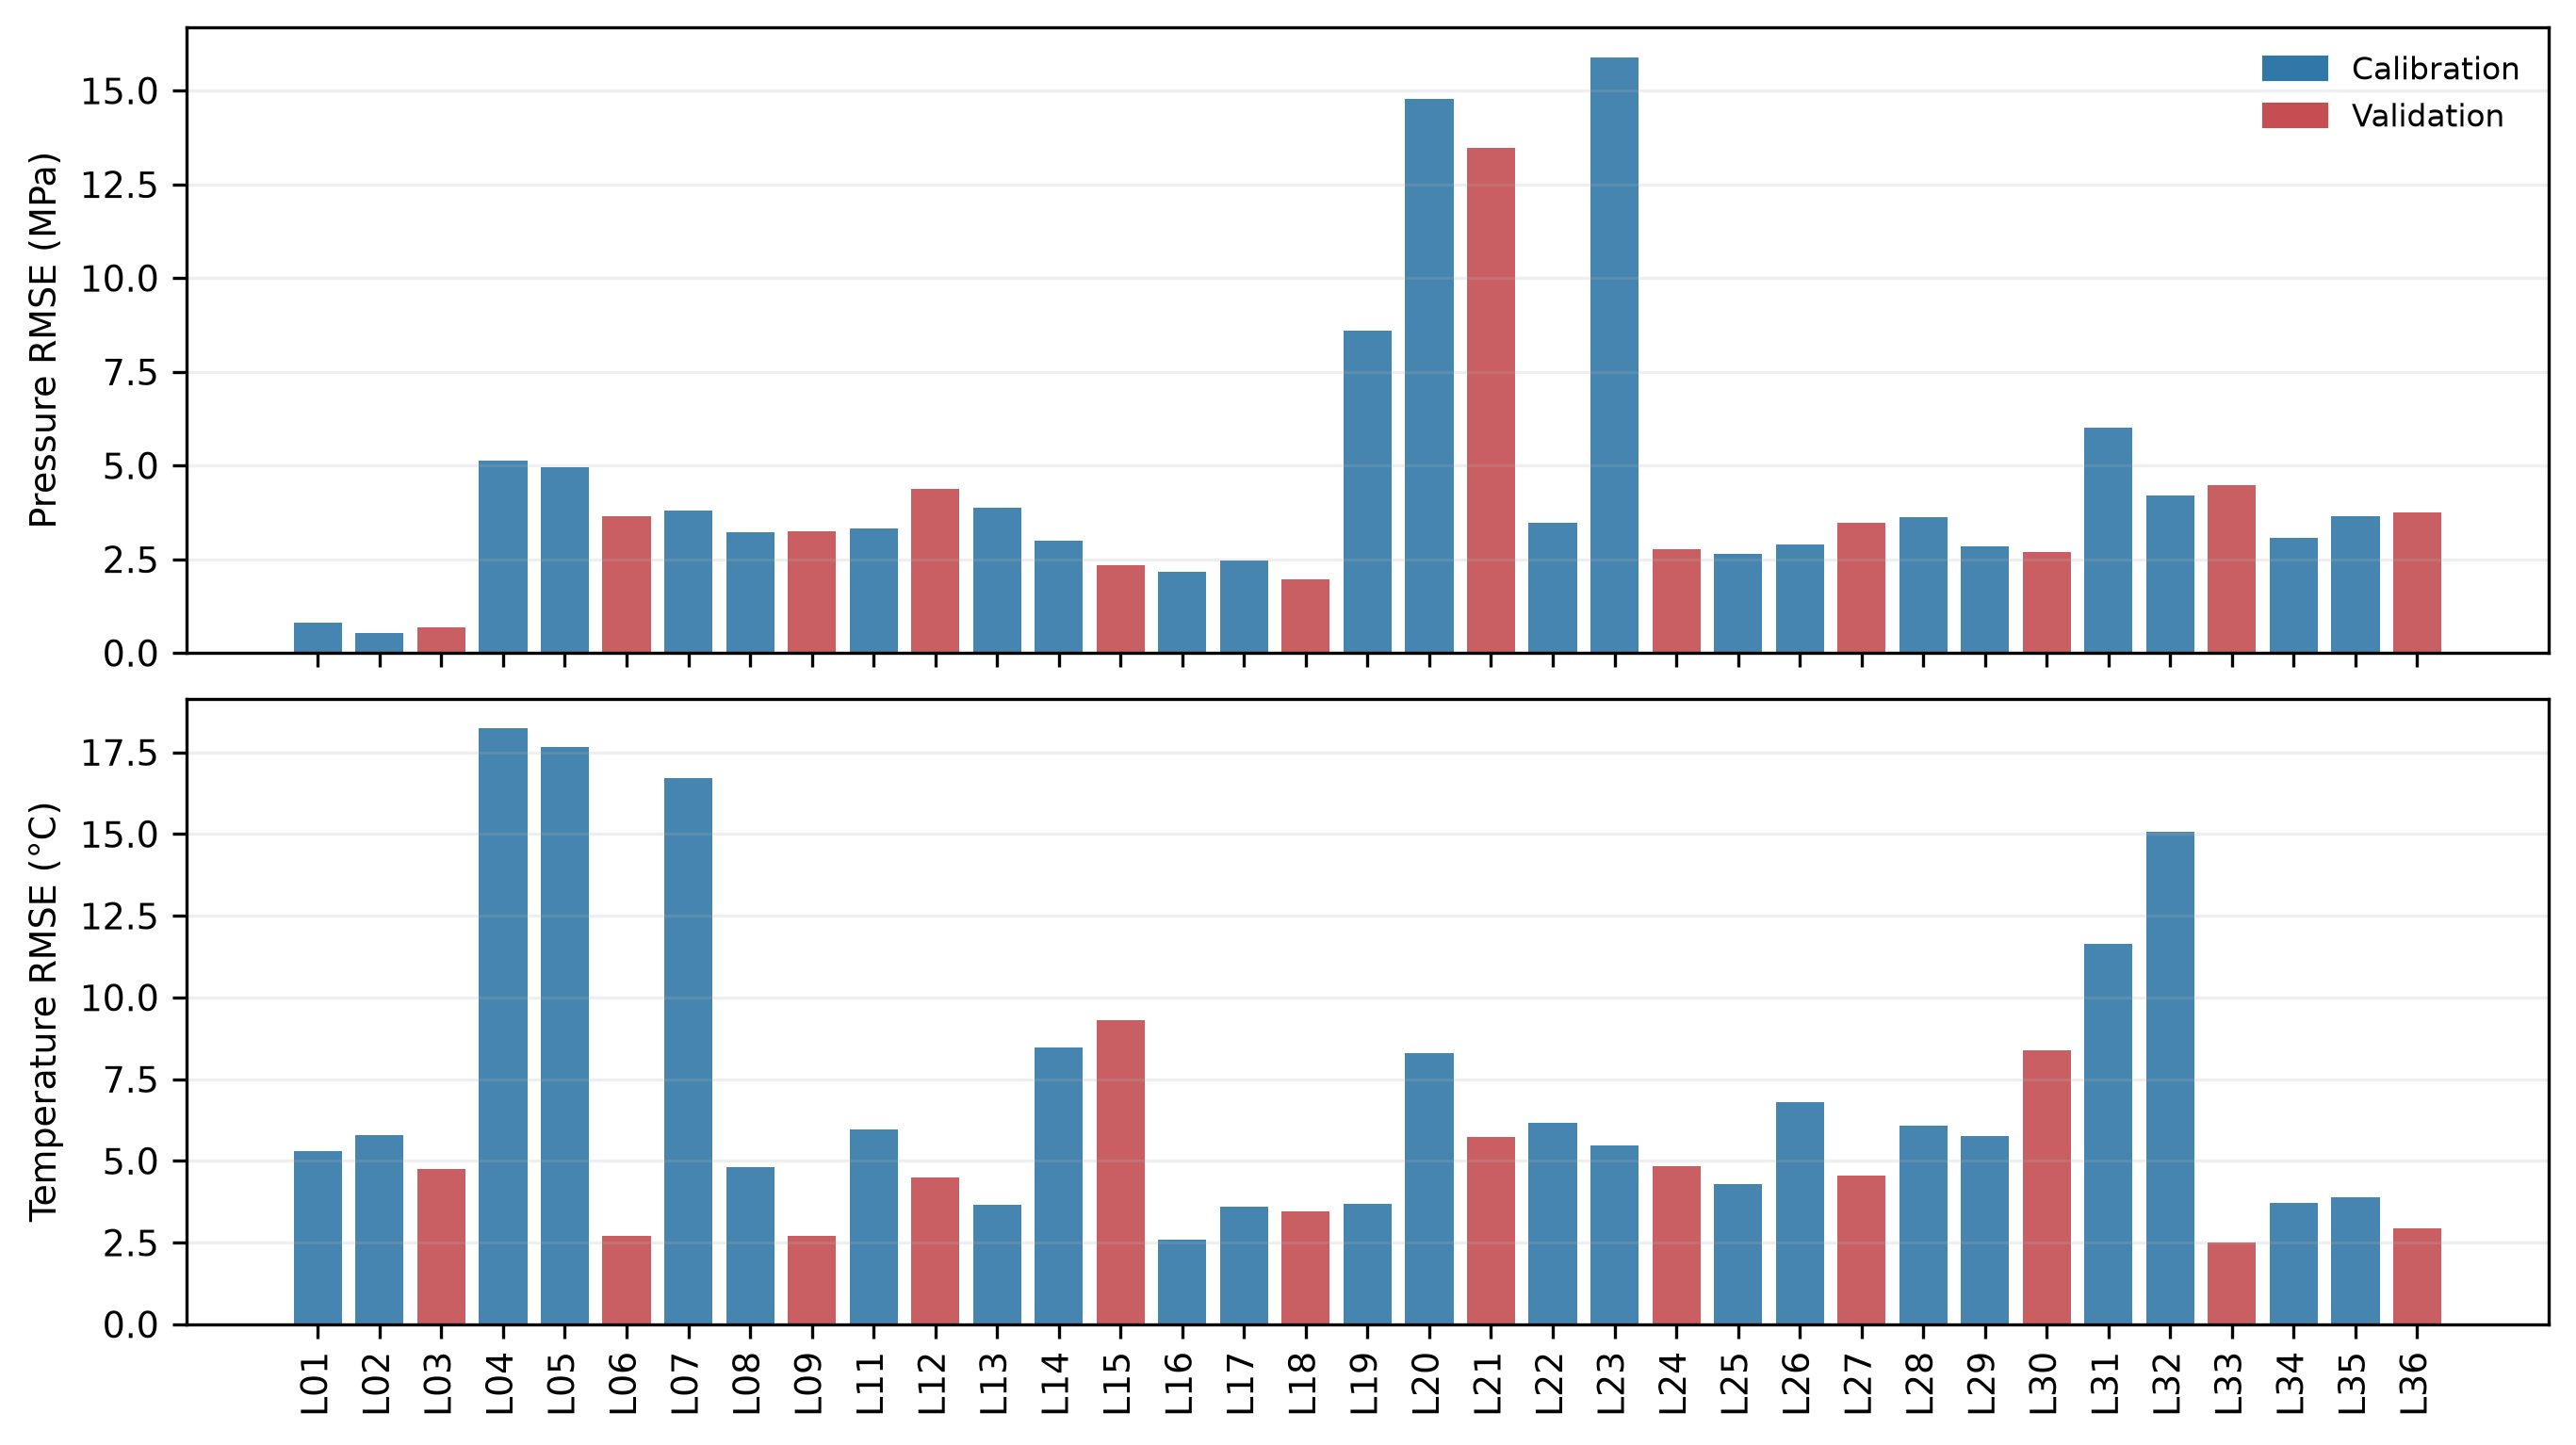
\includegraphics[width=\linewidth]{figures/tank_case_rmse.png}
\caption{Case-level pressure and gas-temperature RMSE. The frozen validation
cases are every third laboratory test; L10 was excluded by the pre-model
mass-closure screen and therefore has no bar.}
\label{fig:cases}
\end{figure}

The fitted gas-to-liner multiplier is large and the optimizer's reported first-
order optimality (3115.9) indicates a shallow or imperfectly resolved optimum even
though its termination flag was successful. The fit should therefore be treated
as an effective heat-transfer calibration, not an identified physical coefficient.

\subsection{Negative full-loop validation result}
After the preprocessing and nominal-pressure corrections, refitted tank, flow-area
calibration and frozen v2 cooling sensitivity, one of eight development fills and
two of eleven internal-comparison fills met all three project screens. Their mean
errors improved to 6.602 MPa, 11.428 $^{\circ}$C and 7.297 SOC percentage points
for development, and 4.530 MPa, 7.819 $^{\circ}$C and 4.625 percentage points for
internal comparison. The low joint pass fractions still constitute a negative
full-loop result.

The prospectively frozen MC Default holdout had already been evaluated with its
pre-correction frozen model and passed zero of eight screens
(Table~\ref{tab:closed}). Mean pressure, temperature and SOC RMSE were 15.862 MPa,
13.230 $^{\circ}$C and 18.082 percentage points, respectively. Five runs terminated
on the model's temperature safety logic; final SOC error was negative in all eight
cases and ranged from $-8.42$ to $-50.79$ percentage points. These outcomes were
not rerun or used to tune the corrected model, so they remain historical external
failure evidence rather than validation of the final configuration.

\begin{table}[htbp]
\centering
\caption{Closed-loop performance. The development and already-inspected comparison
sets use the corrected v2 pipeline; the MC Default set reports its prospectively
frozen historical model and was not reused after correction.}
\label{tab:closed}
\small
\resizebox{\textwidth}{!}{%
\begin{tabular}{lrrrr}
\toprule
Set & Pass/all & Pressure RMSE & Temperature RMSE & SOC RMSE \\
 & & (MPa) & ($^{\circ}$C) & (percentage points) \\
\midrule
Corrected development & 1/8 & 6.602 & 11.428 & 7.297 \\
Corrected internal comparison & 2/11 & 4.530 & 7.819 & 4.625 \\
Prospective MC Default, frozen earlier model & 0/8 & 15.862 & 13.230 & 18.082 \\
\bottomrule
\end{tabular}
}
\end{table}

The measured-boundary tank result therefore cannot be used as validation of the
controller, cascade schedule, precooler or dispenser boundary. The independent
holdout demonstrates that the failure is not confined to the previously inspected
comparison set. Systematic underdelivery and false temperature stops identify the
constant-ramp protocol representation, source hydraulics and precooling boundary
as redesign targets. The bench files observe vehicle and source pressures, flow,
inlet temperature and SOC, but do not expose every internal three-bank valve
command; they therefore cannot by themselves validate all cascade dispatch states.

An outcome-independent source-boundary diagnostic further limits the interpretation.
For the eight MC Default traces, the observed third-source pressure drop was only
1.36--4.91 MPa. An isothermal 0.35-m$^3$ high-bank calculation with the same
transferred masses predicts 30.7--58.6 MPa, while the observed pressure and mass
differences imply conditional connected volumes of 2.74--8.70 m$^3$. The public
files do not identify whether this channel represents a larger connected inventory,
a pressure-regulated upstream boundary, multiple banks or different valve and
thermal behaviour. These conditional volumes are therefore retained as a
diagnostic, not fitted into the production model. A new prospective evaluation
must provide source pressure and temperature as boundary traces or disclose the
bank topology and valve states before internal cascade pressure can be assessed.

A superseded development-only sensitivity first scaled hydrogen--coolant and
chiller conductance by factors 1, 2, 4 and 8 and selected its upper bound. After
the parser, tank-fit, flow and nominal-pressure corrections, a replacement
protocol was frozen before evaluating factors 1, 2, 4, 8, 12 and 16. It again
selected the upper bound, but the normalized objective decreased only from 11.051
at 8 to 10.969 at 16. The retained factor 16 produced the corrected results in
Table~\ref{tab:closed}; larger values were not searched. The upper-bound optimum,
diminishing improvement and remaining case-level failures indicate that cooling
duty alone does not explain the closed-loop error. Neither sensitivity was applied
to the consumed external holdout.

To separate the protection logic from the underlying boundary-model error, a
post-outcome sensitivity reran the same eight traces with both the controller
and safety-PLC vehicle-gas temperature trip raised from 85 to 95~$^{\circ}$C.
This counterfactual produced no screening passes; mean pressure, gas-temperature
and final-SOC RMSE were 10.217~MPa, 14.301~$^{\circ}$C and 12.605 percentage
points, respectively, and none of the cases stopped on the temperature limit.
The diagnostic is therefore evidence that the negative holdout is not explained
solely by premature temperature shutdown. It is explicitly post-outcome,
does not change the frozen decision, and cannot substitute for a new
prospectively frozen holdout with an independently justified safety limit.
The complete run metadata are archived in
\texttt{research/closed\_loop\_temperature\_stop\_diagnostic\_2026\_10\_04.json}.

\subsection{Prospective confined pressure-peaking screen}
To test a separate consequence boundary without presenting it as station-loop
validation, a second prospective protocol was frozen before accessing the raw
outcomes of the HyTunnel-CS unignited pressure-peaking release archive
\cite{lach2020}. The source contains ten synchronized pressure and mass-flow
experiments (cases 2--11) in a 14.9~m$^3$ vented enclosure. The fixed model
used source-documented vent areas and initial temperatures, the measured mass
flow as input, a constant-temperature ideal-gas balance and the fixed
publication value $C_d=0.7$; no case-specific fitting or outcome-based case
selection was permitted.

All ten cases were eligible. Seven passed both predeclared primary screens
(peak overpressure absolute error $\leq5$~kPa and peak-time relative error
$\leq20\%$), giving 70\%. This was below the frozen 80\% confirmatory
threshold, so the result is exploratory evidence for a confined unignited
pressure-peaking submodel only. It does not validate outdoor dispersion,
ignition, emergency response or the complete HRS fueling loop.

\subsection{Negative ambient blowdown validation result}
All 22 PRESLHY workbooks were eligible, spanning four nozzle diameters and low,
medium and high initial-pressure groups. Eleven cases passed both primary screens,
giving a joint pass fraction of 50.0\% (case-bootstrap 95\% CI 31.8--72.7\%), below
the predeclared 70\% criterion. The direct-aperture source-depletion claim is
therefore not supported for this model revision.

Six eligible cases, all in the high-pressure group and initiated at approximately
150 or 200 bar, encountered a retained thermophysical-domain error when the
calculated restriction choking state left the single-phase hydrogen table. They
were counted as failures. Among the 16 numerically completed cases, 11 passed both
screens (68.8\%); this post hoc descriptive fraction does not replace the primary
decision. Joint pass counts were 2/9 at high pressure, 6/7 at medium pressure and
3/6 at low pressure. By aperture they were 2/4, 0/4, 4/7 and 5/7 for 0.5, 1, 2
and 4 mm, respectively. These strata indicate both a runtime-domain limitation
and model-form error rather than one isolated failed workbook.

\subsection{Development revision and negative E5.1 holdout}
Adding documented vessel-wall thermal inertia and real-gas discharge physics
removed calculation failures on the consumed E3.1 set. Twenty of 22 development
cases passed both original screens (90.9\%; case-bootstrap 95\% CI 77.3--100\%).
This improvement cannot validate the revision because the same experiments had
already been examined and used to motivate the model change.

The frozen E5.1 holdout did not confirm the revised claim. Only three of seven
campaign experiments met the primary measured-temperature definition, below the
minimum four. Two of those three passed both screens (66.7\%; bootstrap 95\% CI
0--100\%), also below the 70\% decision threshold. The two successful cases were
4 mm releases near 50 bar absolute; a 2 mm low-pressure case passed the pressure
NRMSE screen (9.04\%) but missed the half-pressure timing screen by 305.7\%.
Two publisher-labelled ambient winter runs had measured pre-release temperatures
of 277.28 and 273.71 K and therefore remained outside the frozen primary window.
The latter and both cryogenic transfer runs triggered the predeclared
significant-pressure-increase integrity check and were retained as failed
evaluations. The publisher explanation labels the 2 mm run as 50 bar, whereas
the workbook metadata and pre-release trace are approximately 5 bar gauge; the
analysis retains the measured state and separately records the nominal label.
The eligibility minimum and performance threshold both failed, so the revised
source-depletion claim is not supported by this holdout.

\subsection{Negative independent 90 MPa mass-flow transfer}
All three INERIS/CEA diameter series met their eligibility minima, with 13, 10
and 12 paired states for 1, 2 and 3 mm, respectively. None passed both screens.
Peak-normalized NRMSE was 16.27\%, 16.01\% and 32.62\%, while median absolute
percentage error was 25.07\%, 15.85\% and 32.88\%. The 1 mm series was generally
underpredicted, whereas overprediction increased for the 2 and 3 mm series.
Adding 101.325 kPa to the plotted pressure did not change any decision, and no
prediction lay inside the narrow digitization interval. Post-outcome descriptive
least-squares effective discharge coefficients were 1.141, 0.657 and 0.533; they
are diagnostics and were not used to rerun or tune the primary result. The 0/3
joint pass count rejects the independently validated high-pressure aperture-flow
claim for the fixed model.

\subsection{Negative Sandia/SRI transient mass-flow transfer}
The Figure 3b digitization supplied 25 unique experimental coordinates. The
locked model passed the NRMSE screen at 5.83\% of measured peak, but median
absolute percentage error was 22.85\% and half-peak-time error was 28.29\%.
Measured and predicted peak flows were 68.38 and 60.67 g s$^{-1}$; measured and
predicted half-peak times were 13.35 and 9.58 s. Because all three screens were
required, the external transient claim is not supported. The lower predicted
peak followed by faster decay is consistent with omitted vessel-wall heat input
and downstream-tube inventory, but that interpretation is diagnostic and no
post-hoc parameter change enters the primary result.

\subsection{Negative Sandia/SRI pressure-decay transfer}
The separate Figure 4 pressure trace supplied 222 unique coordinates. The
locked model reproduced the initial pressure within 0.04\% and passed the
half-pressure-time screen: measured and predicted times were 26.79 and 28.53 s,
for 6.51\% error. It failed the two curve-wide screens. Initial-pressure-
normalized RMSE was 11.58\% and median absolute percentage error was 27.46\%.
The experimental trace lost pressure much faster during the first seconds,
whereas the model later fell below the measured pressure. Because all screens
were required, the external pressure-decay claim is not supported.

\subsection{Positive bounded Ekoto mass-flow transfer}
The Figure 3 digitization supplied 39 unique experimental coordinates. All
three prospectively frozen screens passed: peak-normalized NRMSE was 3.84\%,
median absolute percentage error was 12.79\%, and half-peak-time error was
6.07\%. Measured and predicted peak flows were 0.04483 and 0.05124 kg s$^{-1}$;
measured and predicted half-peak times were 0.506 and 0.537 s. No post-freeze
parameter or code change was made. This supports a bounded source-depletion claim
for the 13.45 MPa, 3.63 L scaled release, not the enclosing warehouse phenomena
or a full refuelling station.

\subsection{HyRAM+ source, tests and adapter parity}
The installed and upstream v6.1 Python sources matched over 38 files with aggregate
SHA-256 \texttt{d5865e1ae7b5c77b985e06b45d7a5607543703c1834fc50f7c5d96f32a0c22de}.
All 47 selected upstream validation tests passed, comprising 803 subtests and seven
expected physics warnings. Production-adapter outputs matched independent public-
API calls for all three parity cases (Table~\ref{tab:hyram}).

\begin{table}[htbp]
\centering
\caption{Station-scale HyRAM+ 6.1 adapter parity. The plume distance is directional.}
\label{tab:hyram}
\small
\resizebox{\textwidth}{!}{%
\begin{tabular}{lrrr}
\toprule
Case & Modelled flow (kg s$^{-1}$) & 4 vol\% distance (m) & Visible flame (m) \\
\midrule
Low bank, 1 mm & 0.016613 & 4.339 & 2.326 \\
Mid bank, 2 mm, cold & 0.108305 & 11.382 & 6.057 \\
High bank, 3 mm, override & 0.296366 & 17.224 & 9.246 \\
\bottomrule
\end{tabular}
}
\end{table}

This result verifies translation, unit handling, coordinate use, contour selection
and output indexing for the installed package. It does not independently repeat
the experiments underlying Sandia's validation report, validate the virtual
station layout or establish an exclusion zone. A public 22-release open-channel
dataset \cite{henriksen2025} was reviewed but was not force-fitted: its downward
4.6 mm jet in a 5.8 m $\times$ 0.9 m $\times$ 0.8 m channel is not geometrically
applicable to the current outdoor free-jet adapter.

The same dataset was nevertheless used for a separate, bounded detector-logic
replay. The measured 29-channel concentration records were passed through the
declared 1.0 vol\% alarm, 2.0 vol\% trip and 0.5 s persistence rule, with a
record-specific sampling-gap reset. All 22 experiments produced at least one
alarm and one trip detection; mean channel coverage was 0.887 and 0.809,
respectively, and the median first detection occurred 10.675 s after filling
started. This result checks deterministic threshold and persistence handling,
not detector response dynamics, placement, ESD effectiveness or an outdoor HRS
dispersion field. The case-level output and archive digests are retained in the
reproducibility record \texttt{dispersion\_detector\_logic\_validation.json}.

\subsection{Decision-support study status}
The deterministic split produces a 24-case holdout casebook and nine development
cases, but all vignettes remain unapproved until coordinator leakage review and
qualified expert sign-off; the institutional ethics determination is also pending.
The pre-outcome sensitivity simulation estimated 77.7\% power at a standardized
paired effect of 0.6 and 95.7\% at 0.8. Even with zero unsafe-advice events among
24 events, the exact two-sided 95\% upper event-rate bound would remain 14.2\%.
Consequently, no SAGA effectiveness, safety, latency,
omission-rate or inter-rater-agreement result is reported in this draft. This empty
result is deliberate: substituting model self-assessment would violate the frozen
protocol.

\section{Discussion}
\subsection{What is externally supported}
The strongest independent result concerns vehicle-tank thermodynamics under
measured inlet mass flow and temperature. It supports use of the tank submodel for
research comparisons within the tested fast-fill envelope, subject to the
effective geometry and heat-transfer assumptions. The result is strengthened by
a deterministic split, experiment-only exclusion rule, global rather than case-
specific fitting, trace alignment on the original clock and case-level bootstrap
intervals.

The complete-loop result is informative precisely because it is negative. A
visually plausible pressure ramp and a stable numerical integration are
insufficient evidence for a station controller. The prospective MC Default result
also shows that freezing the analysis alone cannot rescue a structurally inadequate
protocol representation. The retained failures identify the missing information
needed for the next experiment: dispenser valve command and position, upstream
and downstream pressure at the PCV, delivered-gas temperature, bank-selection
state and high-rate vehicle inlet mass flow. The eight MC Default and eleven
previously inspected comparison cases are now consumed evaluation evidence and
cannot be used as a new holdout. Model redesign must use development evidence or
physical invariants, followed by a separately acquired and pre-frozen external set.

The negative PRESLHY result places an additional boundary on the release path.
The published DisCha vessel weighs about 28 kg, whereas the frozen validation
model deliberately imposed an adiabatic gas control volume with no wall heat
transfer. Deep calculated cooling ultimately left the available restriction-state
domain in six high-pressure cases, and several lower-pressure cases completed but
missed the half-time or pressure screen. A revised model should represent the
documented vessel thermal mass and physically justified gas--wall transfer, extend
the thermophysical domain only where single-phase assumptions remain valid, and
test valve/line dynamics as a separate effect. The 22 cases now constitute consumed
development evidence. Any improved version requires a new hash-locked external
holdout rather than rerating these cases as independent validation.

The E5.1 campaign supplied that prospective test, but it did not rescue the
claim. Its negative decision is driven jointly by the frozen eligibility rule and
performance, not by selective case deletion. The two nominally ambient winter
runs illustrate why measured-state definitions must be fixed prospectively.
Although the remaining two 50 bar, 4 mm cases transferred well, the primary set
was too small and lacked a successful high-pressure case. E5.1 also shares the
DisCha facility and investigators with E3.1, so even a passing result would have
been separate-campaign evidence rather than independent-laboratory replication.

The independent French campaign then exposed a different limitation. A constant
coefficient multiplying nominal aperture area cannot represent the observed
diameter scaling across a 10 m delivery path: the fitted diagnostic coefficient
decreased strongly as diameter increased, while exceeding unity for 1 mm. This
does not justify three new coefficients. It requires an explicit valve--pipe--
orifice network, geometric uncertainty and a new untouched facility for testing.
The Proust curves are now consumed development evidence. Their plot-digitization
uncertainty was much smaller than the discrepancies and did not determine the
negative result.

A post-outcome network diagnostic illustrates why a universal fitted correction
would be misleading. A series-conductance approximation selected on the consumed
Proust curves (2.62 mm equivalent upstream restriction) brought all three Proust
diameter groups inside the descriptive error screens, but its NRMSE increased to
29.25\% and 41.81\% on the already-visible 3 and 4 mm Imamura series. A direct
aperture relation with $C_d=1.0$ instead remained between 3.79\% and 7.60\%
NRMSE across the consumed 1--4 mm Imamura data. Because both outcome sets were
visible before this comparison was formalized, these numbers are development
diagnostics only. They indicate apparatus-specific valve or upstream resistance
rather than a transferable nozzle correction and leave the negative Proust
decision unchanged.

The separate Sandia/SRI transient reinforces the thermal limitation without
sharing the PRESLHY or INERIS/CEA facilities. Its low aggregate NRMSE can obscure
the operationally relevant timing error: the adiabatic vessel model depleted the
flow too quickly. A non-adiabatic two-cylinder wall model and explicit 7.6 m tube
line-pack are therefore development priorities. The Figure 3b trace is now
consumed evidence, and the known approximate duration prevents describing this
test as fully blinded.

The 2007 pressure trace makes the omitted dynamics more specific. A single
adiabatic vessel state could match the initial value and half-pressure time while
still missing both the rapid initial manifold transient and the heat-supported
late tail. This experiment is now consumed evidence. It motivates explicit
valve/manifold line-pack and wall thermal inertia, followed by a new facility-
level holdout rather than post-hoc adjustment of the failed result.

The Ekoto holdout shows that the unchanged model is useful within a narrower
regime: a short, small-inventory 13.45 MPa release with independently specified
$C_d$. Its joint pass does not resolve the failed 15.5 MPa long-tail mass-flow,
43.1 MPa pressure-decay or 90 MPa diameter-scaling tests. Reporting the positive
and negative transfers together defines the model's present applicability more
credibly than a single validation curve.

\subsection{Consequence calculations and risk communication}
The HyRAM verification separates source identity, upstream physics tests and local
adapter parity. The traceability chain covers three geometrically applicable public
experimental families: Han et al.'s 4 vol\% dilution length \cite{han2013},
Schefer--Houf distance-dependent heat flux \cite{houf2007}, and published
unconfined-overpressure distance series summarized in the HyRAM validation report
\cite{hyram2024}. The
browser now renders the first as a directional tapered plume and the latter two as
an equipment-footprint-centred sampled screening band. This supports a bounded
outdoor free-jet display claim. It does not establish a site-specific contour or
justify interpreting the last sampled 5 kW m$^{-2}$/5 kPa point as a legally
sufficient setback. Choked-flow cases may cause HyRAM to recompute mass flow from
source pressure, temperature, aperture and discharge coefficient; both requested
and modelled flows must remain visible in any reported result.

An independent public consequence archive was also prospectively reserved for an
ignited-release thermal screen. Lach and Gaathaug's CC BY 4.0 Figshare record
contains all eight MAT experiments from real-scale 350/700 bar releases through
0.5/1.0 mm TPRD outlets in a semi-confined, mechanically ventilated space
\cite{lachgaathaug2022}. The frozen protocol retains every public experiment and
predeclares time-resolved temperature, heat-flux and release-timing observables;
it does not select cases after inspecting outcomes. The archive is relevant to
thermal-consequence boundary checks, but it is not a station-to-vehicle fill
trace and cannot establish site-specific separation distances, controller
performance or emergency-response effectiveness. The file-selection and claim
boundary are recorded in
\texttt{research/thermal\_effects\_ignited\_release\_protocol\_2026\_10\_04.json};
raw MAT files remain external to preserve the source's attribution and repository
size constraints.

After the freeze, all eight MAT files were replayed with the same descriptive
extractor. The deterministic mass-flow window gave initial tank pressures of
355--703 bar and peak mass flows of 4.04--13.00 g s$^{-1}$; the four radiative
heat-flux channels covered peak ranges of 0.30--1.63, 0.22--11.90,
0.020--0.958 and 0--57.29 kW m$^{-2}$, respectively. These values are retained
as an auditable consequence-data summary, not as a fitted model score: the public
file metadata do not provide an experiment-to-nozzle-angle mapping or a complete
confined CFD boundary. The replay therefore strengthens source provenance and
observability while leaving the station-loop and consequence-model validation
gates unchanged.

\subsection{Evidence-gated language-model assistance}
The LLM is positioned after deterministic calculations and receives structured
sensor provenance, scenario status, consequence fields and uncertainty flags.
This order prevents text generation from fabricating a missing damage radius.
The planned three-arm incident study separates the effects of language generation
and standards retrieval. Its primary value will depend on qualified blinded
ratings, unsafe-advice and critical-omission rates, not stylistic preference.
Until those data exist, SAGA remains an interface and study hypothesis.

\subsection{Limitations}
All live sensors, valves, CCTV views and operator actions are simulated. No field
PLC, dispenser, gas detector or station historian has been connected. Vessel
geometry is inferred from nominal capacity scaling. The tank is lumped and cannot
resolve local hot spots. Compressor maps, valve coefficients, thermal hardware,
weather, occupancy and site geometry are scenario assumptions. The public J2601
archives do not supply the complete proprietary protocol implementation. HyRAM
outputs are conditional consequences, not certification; buildings, congestion,
terrain and site-specific wind are not resolved, and no site field campaign was
performed. The HIAD narratives are
retrospective and may contain incomplete or heterogeneous reporting. Finally,
the original direct-aperture model and its prospectively evaluated non-adiabatic
revision failed their respective PRESLHY claim rules. The fixed aperture relation
also failed all three eligible independent 90 MPa mass-flow series, and the SAGA
study has no locked expert ratings yet. The independent Sandia/SRI mass-flow and
pressure-decay transients each passed only one of three required screens.
The separate Ekoto scaled release passed all three screens but covers only a
small, short-duration source. The public ELVHYS 4.2 archive provides valuable
cryogenic transfer-connection-space pressure-peaking observations, but the
post-access replay in this study is limited to source-file and timebase
integrity; it is not predictive validation of the gaseous H70 station loop
because it lacks vehicle-side and controller telemetry \cite{elvhys2025}.

\section{Conclusions}
A hydrogen-station safety digital twin was evaluated with separate evidence gates
for component physics, full-loop behavior, consequence-software translation and
LLM decision support. The measured-boundary Type-IV tank model achieved validation
mean RMSE values of 3.841 MPa, 4.833 $^{\circ}$C and 3.850 SOC percentage points.
The complete loop did not meet the declared screens, even after structural defects
and preprocessing errors were corrected; only 1/8 development and 2/11 internal
comparison fills passed, and a prospectively frozen earlier eight-case external
holdout passed zero screens. The frozen ambient blowdown model also failed its
prospective external test: 11/22 cases passed both screens and six eligible
high-pressure cases produced retained thermophysical-domain failures. Although
the non-adiabatic revision passed 20/22 consumed development cases, its frozen
E5.1 holdout was ineligible and negative: only three cases met the primary
temperature window and 2/3 passed both screens. An independent 90 MPa Type-IV
release campaign passed zero of three mass-flow series, exposing diameter-
dependent network resistance absent from the aperture-only model. The separate
25-point Sandia/SRI transient passed its 5.83\% NRMSE screen but failed median-
error (22.85\%) and half-peak-time (28.29\%) screens, independently showing that
the adiabatic source depletes too quickly. A separate 222-point 43.1 MPa
pressure-decay holdout passed only its half-time screen (6.51\% error), while
NRMSE (11.58\%) and median error (27.46\%) failed. The 39-point Ekoto scaled
release passed all three frozen mass-flow screens, with 3.84\% NRMSE, 12.79\%
median error and 6.07\% half-time error. This positive result remains bounded to
its 13.45 MPa, 3.63 L source. A prospectively specified KIT 20 MPa pressure-
decay test remained ineligible because the accessible low-resolution publisher
raster did not separate the measured half-pressure crossing; its 51-point
startup segment is retained without a validation claim. The HyRAM+ adapter reproduced the installed v6.1
public API while
the identical upstream source passed its available validation tests; a frozen
browser contract retained the experimentally corresponding directional and radial
geometry semantics. The incident
decision-support experiment is specified but incomplete. These results support a
reproducible research prototype and a disciplined validation workflow; they do
not support claims of SAE-compliant fuelling control, field safety certification
or autonomous emergency management.

\section*{Data and code availability}
Source code, study scripts, frozen machine-readable evidence and documentation are
available under the MIT License at
\url{https://github.com/lyullee/hydrogen-station-sim}; archived release DOI:
\href{https://doi.org/10.5281/zenodo.23084421}{10.5281/zenodo.23084421}.
Third-party raw archives are not redistributed where their terms do not provide a
redistribution licence. The repository records landing pages, checksums, acquisition
instructions, split rules and analysis seeds. HyRAM+ remains governed by its own
GPL-3.0 licence. The eventual SAGA study archive must include masked responses,
locked ratings and the allocation key without API credentials.

\section*{CRediT authorship contribution statement}
\textit{To be completed by the authors before submission.}

\section*{Declaration of competing interest}
\textit{To be completed and approved by every author before submission.}

\section*{Funding}
\textit{Funding source and grant number, or a no-specific-funding statement, must
be confirmed before submission.}

\section*{Acknowledgements}
\textit{Institutional and technical acknowledgements to be confirmed.}

\section*{Declaration of generative AI and AI-assisted technologies in the
manuscript preparation process}
During preparation of this working draft, the authors used OpenAI Codex to assist
with drafting, structure and formatting. The authors must review and edit all
content, references and claims before submission and take full responsibility for
the final article.

\begin{thebibliography}{99}
\bibitem{schneider2014}
J. Schneider et al., Validation and sensitivity studies for SAE J2601,
\textit{SAE International Journal of Alternative Powertrains} 3(2) (2014),
\href{https://doi.org/10.4271/2014-01-1990}{doi:10.4271/2014-01-1990}.

\bibitem{kuroki2021}
T. Kuroki et al., Thermodynamic modeling of hydrogen fueling process from high
pressure storage tanks to vehicle tank, \textit{International Journal of Hydrogen
Energy} 46 (2021) 22004--22017,
\href{https://doi.org/10.1016/j.ijhydene.2021.04.037}{doi:10.1016/j.ijhydene.2021.04.037}.

\bibitem{rothuizen2013}
E. Rothuizen et al., Optimization of hydrogen vehicle refueling via dynamic
simulation, \textit{International Journal of Hydrogen Energy} (2013),
\href{https://doi.org/10.1016/j.ijhydene.2013.01.161}{doi:10.1016/j.ijhydene.2013.01.161}.

\bibitem{rothuizen2020}
E. Rothuizen et al., Dynamic simulation of the effect of vehicle-side pressure
loss of hydrogen fueling process, \textit{International Journal of Hydrogen Energy}
(2020), \href{https://doi.org/10.1016/j.ijhydene.2020.01.071}{doi:10.1016/j.ijhydene.2020.01.071}.

\bibitem{xiao2024}
J. Xiao et al., Thermodynamic and heat transfer models for refueling hydrogen
vehicles: formulation, validation and application, \textit{International Journal
of Hydrogen Energy} (2024),
\href{https://doi.org/10.1016/j.ijhydene.2023.06.081}{doi:10.1016/j.ijhydene.2023.06.081}.

\bibitem{hyram2024}
Sandia National Laboratories, \textit{HyRAM+ Version 5.1.1 Physics Validation},
SAND2024-14886 (2024), \url{https://www.osti.gov/biblio/2480221}.

\bibitem{hyram2025}
Sandia National Laboratories, \textit{HyRAM+ Technical Reference Manual},
SAND2025-04942 (2025),
\href{https://doi.org/10.2172/2563814}{doi:10.2172/2563814}.

\bibitem{preslhy2023}
T. Jordan, A. Friedrich, A. Veser, N. Kotchourko, \textit{PRESLHY Experiment
series E3.1 (Cryogenic Hydrogen Blow-down/Discharge) results--part A high
pressure}, Karlsruhe Institute of Technology (2023),
\href{https://doi.org/10.35097/1187}{doi:10.35097/1187}.

\bibitem{preslhye5}
T. Jordan, A. Friedrich, A. Veser, N. Kotchourko, \textit{PRESLHY Experiment
series E5.1 (Ignited Discharge) results---Benchmarking}, Karlsruhe Institute of
Technology (2021),
\href{https://doi.org/10.35097/1258}{doi:10.35097/1258}.

\bibitem{proust2011}
C. Proust, D. Jamois, E. Studer, High pressure hydrogen fires,
\textit{International Journal of Hydrogen Energy} 36(3) (2011) 2367--2373,
\href{https://doi.org/10.1016/j.ijhydene.2010.04.055}{doi:10.1016/j.ijhydene.2010.04.055}.

\bibitem{schefer2006}
R.W. Schefer, W.G. Houf, B. Bourne, J.D. Colton, Spatial and radiative properties
of an open-flame hydrogen plume, \textit{International Journal of Hydrogen
Energy} 31(10) (2006) 1332--1340,
\href{https://doi.org/10.1016/j.ijhydene.2005.11.020}{doi:10.1016/j.ijhydene.2005.11.020}.

\bibitem{schefer2007}
R.W. Schefer, W.G. Houf, T.C. Williams, B. Bourne, J. Colton,
Characterization of high-pressure, underexpanded hydrogen-jet flames,
\textit{International Journal of Hydrogen Energy} 32(12) (2007) 2081--2093,
\href{https://doi.org/10.1016/j.ijhydene.2006.08.037}{doi:10.1016/j.ijhydene.2006.08.037}.

\bibitem{ekoto2012}
I.W. Ekoto, E.G. Merilo, W.G. Houf, G.H. Evans, M.A. Groethe,
Experimental investigation of hydrogen release and ignition from fuel cell
powered forklifts in enclosed spaces, \textit{International Journal of Hydrogen
Energy} 37(22) (2012) 17446--17456,
\href{https://doi.org/10.1016/j.ijhydene.2012.03.161}{doi:10.1016/j.ijhydene.2012.03.161}.

\bibitem{han2013}
S.H. Han, D. Chang, J.S. Kim, Release characteristics of highly pressurized
hydrogen through a small hole, \textit{International Journal of Hydrogen Energy}
38(8) (2013) 3503--3512,
\href{https://doi.org/10.1016/j.ijhydene.2012.11.071}{doi:10.1016/j.ijhydene.2012.11.071}.

\bibitem{houf2007}
W.G. Houf, R.W. Schefer, Predicting radiative heat fluxes and flammability
envelopes from unintended releases of hydrogen, \textit{International Journal of
Hydrogen Energy} 32(1) (2007) 136--151,
\href{https://doi.org/10.1016/j.ijhydene.2006.04.009}{doi:10.1016/j.ijhydene.2006.04.009}.

\bibitem{henriksen2025}
M. Henriksen, H.E. Fossum, E. Akervik, D. Bjerketvedt, Experimental data of
hydrogen dispersion in an open-ended rectangular channel, version 2 (2025),
\href{https://doi.org/10.23642/usn.26117989.v2}{doi:10.23642/usn.26117989.v2}.

\bibitem{hiad2026}
European Commission Joint Research Centre, \textit{European Hydrogen Incidents
and Accidents Database, HIAD 2.2}, Petten, The Netherlands (accessed 2026).

\bibitem{khk2026}
High Pressure Gas Safety Institute of Japan, \textit{Hydrogen-related accident
information}, public accident-report inventory (accessed 2026),
\href{https://www.khk.or.jp/hydrogen/accident_information.html}{KHK public
report page}.

\bibitem{caponi2022}
R. Caponi, A. Monforti Ferrario, E. Bocci, K. Fl\o che Juelsgaard, Four years
of operational data for five hydrogen refueling stations, \textit{E3S Web of
Conferences} 334 (2022) 06008,
\href{https://doi.org/10.1051/e3sconf/202233406008}{doi:10.1051/e3sconf/202233406008}.

\bibitem{lachgaathaug2022}
A. Lach, A.V. Gaathaug, \textit{Experimental data--hydrogen safety, thermal
effects}, University of South-Eastern Norway / Figshare (2022),
\href{https://doi.org/10.23642/usn.17695082.v1}{doi:10.23642/usn.17695082.v1}.

\bibitem{lach2025thermal}
A.W. Lach, K. Vaagsaether, A.V. Gaathaug, Thermal hazards from a downwards
hydrogen impinging jet--real scale experimental results from up to 700 bar
pressure releases in a carpark, \textit{International Journal of Hydrogen
Energy} 116 (2025) 420--429,
\href{https://doi.org/10.1016/j.ijhydene.2025.03.121}{doi:10.1016/j.ijhydene.2025.03.121}.

\bibitem{lach2020}
M. Lach et al., Unignited pressure peaking phenomena, \textit{International
Journal of Hydrogen Energy} (2020),
\href{https://doi.org/10.1016/j.ijhydene.2020.08.221}{doi:10.1016/j.ijhydene.2020.08.221};
data record: \href{https://doi.org/10.5281/zenodo.4106101}{10.5281/zenodo.4106101}.

\bibitem{elvhys2025}
W. Rattigan, J. Welch, J. Vizma, \textit{ELVHYS 4.2 -- Leakage into cold
room/tank connection space considering barriers and obstacles}, HSE / NTNU
DataverseNO (2025), \href{https://doi.org/10.18710/JXJP0H}{doi:10.18710/JXJP0H}.

\bibitem{iso19880}
ISO, \textit{ISO 19880-1:2020 Gaseous hydrogen---Fuelling stations---Part 1:
General requirements}, International Organization for Standardization (2020).

\bibitem{saej2601}
SAE International, \textit{SAE J2601: Fueling Protocols for Light Duty Gaseous
Hydrogen Surface Vehicles}, 2020 edition.

\bibitem{nrc2024}
L. Zhang, Y. Wang, C. Dec\'es-Petit, \textit{Dispenser reliability analysis for
hydrogen refuelling stations in British Columbia}, National Research Council
Canada, Report 56628 (2024),
\href{https://doi.org/10.4224/40003368}{doi:10.4224/40003368}.

\bibitem{prhyde2023}
PRHYDE Consortium, \textit{PRHYDE Results as Input for Standardisation},
Deliverable D6.7 Rev. 1.2 (2023),
\href{https://lbst.de/wp-content/uploads/2023/04/PRHYDE_Deliverable-D6-7_Results_as_Input_for_Standardisation_V1-2_final_Apr_2023.pdf}{public
deliverable}.

\bibitem{monde2012}
M. Monde, P. Woodfield, T. Takahashi, M. Ishimoto, Estimation of temperature
change in practical hydrogen pressure tanks being filled at high pressures of
35 and 70 MPa, \textit{International Journal of Hydrogen Energy} 37 (2012)
5723--5734,
\href{https://doi.org/10.1016/j.ijhydene.2011.12.136}{doi:10.1016/j.ijhydene.2011.12.136}.
\end{thebibliography}

\end{document}
